\section{Introduction}
\label{sec:introduction}



In this chapter, we address the problem of finding a suitable cloud
VM type for a recurring job.
This problem is further aggravated by
the \textit{long execution times of the workloads} since a brute-force approach will no longer be a viable option.
Furthermore, because there are evaluation costs, this
\emph{decision space} must be explored efficiently.
The prior work in this area, solved this problem using two different approaches namely (1)
\emph{PARIS}~\cite{Yadwadkar2017} builds a complex performance model (using
large-scale one-time benchmark data) to predict workload performance, and
(2) \emph{CherryPick}~\cite{Alipourfard2017} uses Bayesian optimization to find the best cloud configuration.
We prefer the Bayesian Optimization (BO) method because
it does not require additional historical training data and
supports any objective functions (essential for diverse workloads).


\begin{figure}[!htbp]
    \centering
    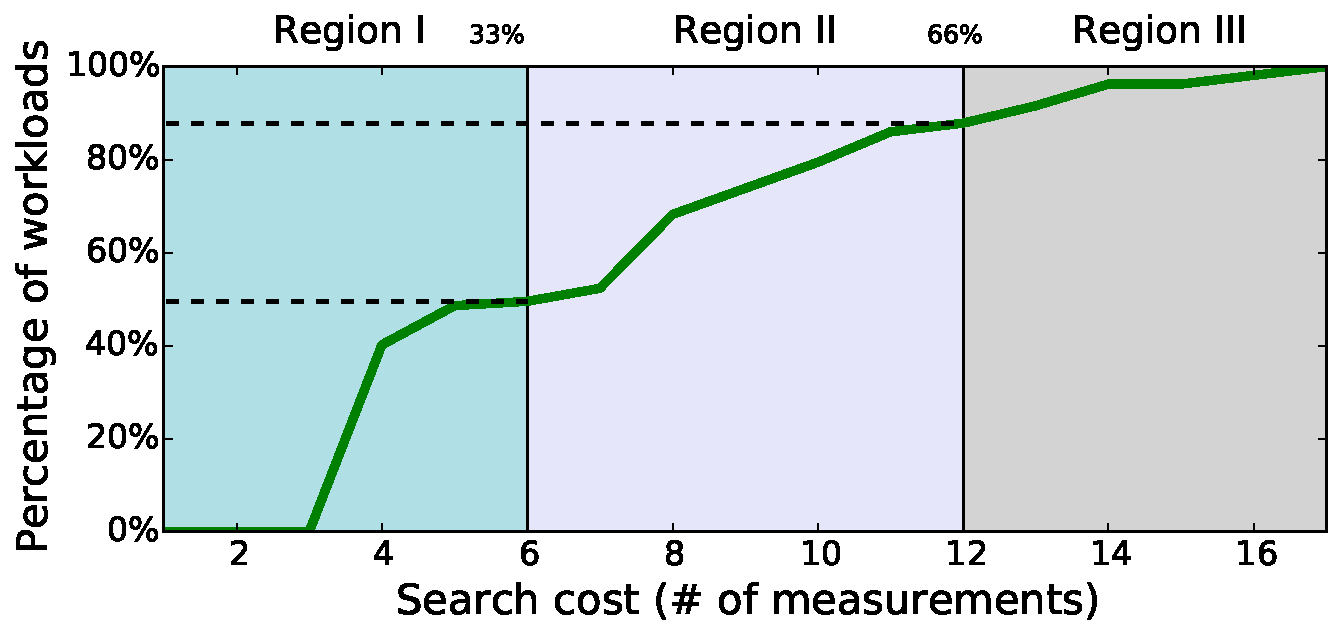
\includegraphics[width=0.8\textwidth]{figures/motivation_fragile_cost.pdf}
    \caption{The number of measurements required by Bayesian Optimization (as used in ~\cite{Alipourfard2017}) to find the optimal VM type. We observe that 50\% and 85\% of the workloads (shown in dashed lines) require 6 (33\% of the search space) and 12 (66\% of the search space) measurements respectively. Bayesian Optimization is not always effective for any workload.
    The fragility problem---either incurs high search cost or yields sub-optimal solution (as in \emph{Region II} and \emph{Region III}).}
    \label{fig:cherrypick_issue1}
\end{figure}


However, we have come across workloads where a \bo method is ineffective---surprisingly,
we found this problem in a large number of workloads.
Our large-scale empirical study, as shown in \myfigure{~\ref{fig:cherrypick_issue1}},
reveals that BO incurs different search cost on different workloads.
We observe that \bo is effective in 50\% of the workloads (in \emph{Region I}) since it requires exploration of only
33\% of the total search space.
However, we also notice that \bo is not as effective at finding the optimal VM type
for the other workloads (in \emph{Region II} and \emph{Region III}).
This poor performance can be attributed to
the insufficient information (for example core counts, memory capacity, etc.) used by \bo during the search process.
Such VM characteristics are not sufficient to capture application behavior~\cite{Hsu2016, Yadwadkar2017, Dalibard2017}.
Consequently, \bo may fail to find the optimal VM for some workloads efficiently.
Figure~\ref{fig:cherrypick_issue2} shows
how \bo is sluggish to find a `better' VM type for a workload from the \emph{Region III}.
In summary, the lesson that we learned from the large-scale empirical study is \textit{\bo is not a silver bullet to find optimal VM type} for any workloads.
Furthermore, it can be \textit{fragile}---either incurs higher search cost or yields a sub-optimal solution.
Without further investigation, it is hard to claim BO is an effective method for finding the best VM type.


To further understand the fragility of Bayesian Optimization,
we conducted a large-scale empirical study with three popular big data systems along with 107 different workloads and 18 different VM types
(for more details refer to Section~\ref{sec:cat::dataset}).  
We first observe that using rules-of-thumb (intuitions) to select the best VM type is far from ideal.
There does not exist one such best VM type for all the workloads.
Second, the same application with different input sizes may favor different VM types.
Last,
while the execution time tends to decrease with a more powerful
VM, the cost per unit time goes up, which compresses the
deployment costs.
This creates a \textit{level playing field}---several inferior
configurations in execution time are now competitive in deployment cost.
These reasons make the problem of selecting the best VM for any given workload challenging.
% These are the challenges of selecting a well-suited VM type for a given workload.

To find the best VM type, \emph{CherryPick}~\cite{Alipourfard2017} uses Bayesian Optimization, which sequentially evaluates the VMs and
moves closer to the optimal VM type.
As presented before, a BO method can encounter the fragility problem.
As shown in Figure~\ref{fig:cherrypick_issue2}, 
the execution time on the selected instance type after the fifth iteration is 1.75 times slower when
compared to the optimal instance type.
In this case, BO did not find the optimal solution until the thirteenth attempt.
We argue that the fragility of BO arises from the \textit{insufficient information}.
That is, characteristics of a VM such as CPU speed, core counts, memory per core and disk capacity, are not sufficient to predict its performance.
Besides, the \textit{choice of the kernel function} (the prior) and
the selection of the initial measurements are both critical to the effectiveness of BO~\cite{Brochu2010, Snoek2012, Dewancker2015, shahriari2016taking}.
We believe they are also related to the fragility problem.


\begin{figure}[!htbp]
    \centering
    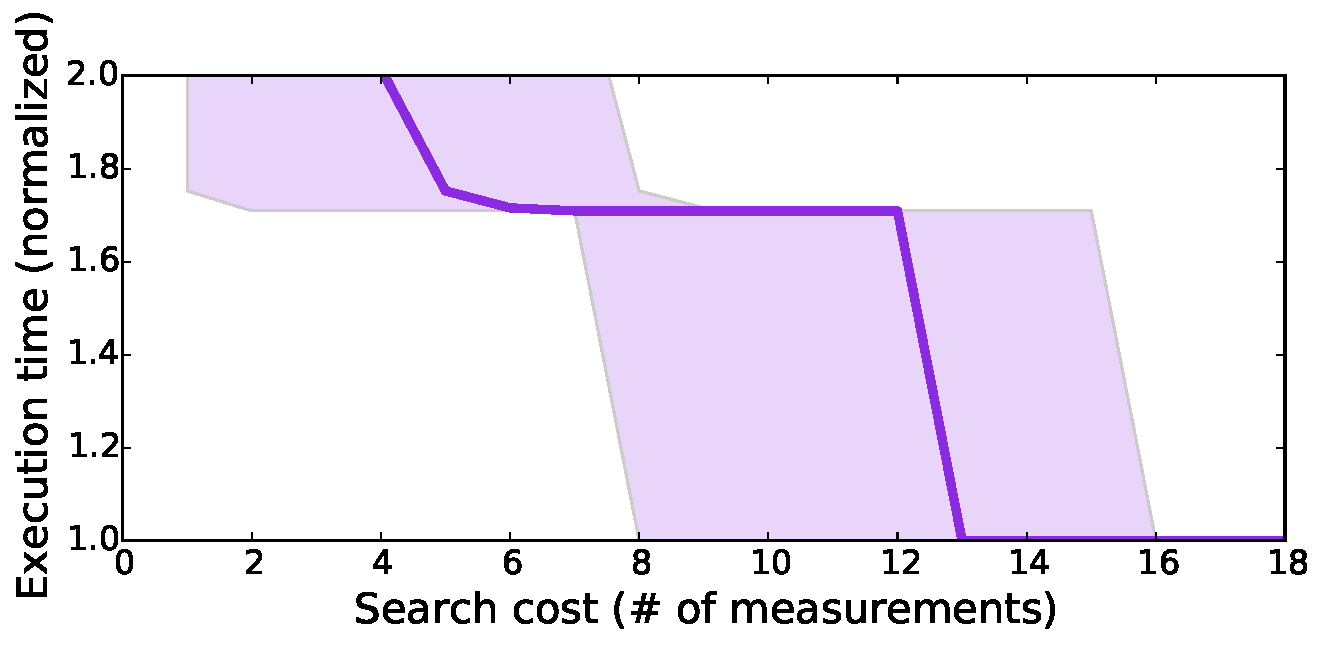
\includegraphics[width=0.8\textwidth]{figures/cherrypick_issue_spark_als_large_new.pdf}
    \caption{Using Bayesian Optimization to find the best VM type for running the ALS algorithm on Spark.
    The horizontal axis represents the search cost, and the vertical axis represents the execution time of the workload (for both lower is better).
    The edges of the colored area represents the 25 and the 75 percentile of the execution time.
    A naive Bayesian Optimization method progresses slowly towards the optimal VM type.
    The low-level augmented BO method alleviates the fragility problem as shown in Figure~\ref{fig:convergence_time_1}.
    }
    \label{fig:cherrypick_issue2}
\end{figure}


Low-level performance metrics are a good proxy for estimating
application and system performance~\cite{Hsu2016, Yadwadkar2017}.
They are also useful to identify performance anomalies
~\cite{Bodik2010, Novakovic2013}.
We argue that \textit{low-level performance
  information} such as I/O wait and memory usage well characterizes
application behavior and better
guides a BO method through the search process.

In this chapter, we propose
a novel method to augment Bayesian Optimization
by leveraging low-level performance information.
However, embedding low-level performance information is tricky because the (low-level) information is not available until the workload is executed on a given VM type.
Our proposed modeling technique seamlessly integrates
the high-level features with the low-level performance information.
The prediction model estimates the workload performance
in VMs (not measured) using the
low-level performance information collected from previous measurements.
Throughout the search process, the model keeps updating its belief
based on the new measurements.

The proposed low-level augmented Bayesian Optimization (Augmented BO) outperforms
the naive Bayesian Optimization (Naive BO)~\cite{Alipourfard2017}.
Our evaluation shows a reduction in search cost on 46 out of 107 applications
in search for the most cost-effective configuration.
Our method reduces about 20\% search cost on average for cases
with the fragility issue, and reaches 43\% reduction for some
while maintaining the same or slightly better performance
in comparison to Naive BO.